\documentclass[aip, pop, preprint]{revtex4-1}

\usepackage{graphicx}%
\usepackage{dcolumn}%
\usepackage{bm}%

\usepackage[utf8]{inputenc}
\usepackage{amssymb}
\usepackage{placeins}
\usepackage{amsmath}
\usepackage{amsthm}
\usepackage{commath}
\usepackage[citecolor=blue,colorlinks=true,linkcolor=blue]{hyperref}
\usepackage[margin=1in]{geometry}

\renewcommand{\thefigure}{\thesection.\arabic{figure}}
\renewcommand{\theequation}{\thesection.\arabic{equation}}
\numberwithin{figure}{section}
\numberwithin{equation}{section}

\newcommand{\partder}[2]{\dfrac{\partial  #1}{\partial  #2}} % partial der.
\newcommand{\der}[2]{\dfrac{d #1}{d  #2}}

\begin{document}
\title{Rotation and Neoclassical Ripple Transport in ITER}
\author{E. J. Paul}
\affiliation{Department of Physics, University of Maryland, College Park, MD 20742, USA}
\email{ejpaul@umd.edu}

\author{M. Landreman}
\affiliation{Institute for Research in Electronics and Applied Physics, University of Maryland, College Park, MD 20742, USA}
\email{mattland@umd.edu}

\author{W. Dorland}
\affiliation{Department of Physics, University of Maryland, College Park, MD 20742, USA}
\email{bdorland@umd.edu}

\author{F. M. Poli}
\affiliation{Princeton Plasma Physics Laboratory, Princeton, NJ 08543, USA}
\email{fpoli@pppl.gov}

\author{D. A. Spong}
\affiliation{Oak Ridge National Laboratory, Oak Ridge, TN 37831, USA}
\email{spongda@ornl.gov}

\author{H. M. Smith}
\affiliation{Max-Planck-Institut f\"{u}r Plasmaphysik, 17491 Greifswald, Germany}
\email{hakan.smith@ipp.mpg.de}

\begin{abstract}

Neoclassical transport in the presence of non-axisymmetric magnetic fields causes a toroidal torque known as neoclassical toroidal viscosity (NTV). The toroidal symmetry of ITER will be broken by the finite number of toroidal field coils and by ferromagnetic structures such as test blanket modules (TBMs) and ferritic inserts (FIs). 3D magnetic equilibria are calculated for an ITER steady-state scenario using the Variational Moments Equilibrium Code (VMEC), and neoclassical transport quantities in the presence of these error fields are calculated using the Stellarator Fokker-Planck Iterative Neoclassical Solver (SFINCS). As NTV is a complicated nonlinear function of $E_r$, we study its behavior over a plausible range of $E_r$. We estimate the toroidal flow, and hence $E_r$, using a semi-analytic turbulent intrinsic rotation model and NUBEAM calculations of neutral beam torque. The magnitude of NTV torque density at large radii ($r/a \gtrsim$ 0.6) is comparable to the NBI torque density at small radii ($r/a \lesssim$ 0.4), but is opposite in direction and may significantly damp rotation in the edge. The FIs decrease neoclassical transport, while the TBMs do not produce significant NTV torque. 
\end{abstract}

\maketitle

\section{Introduction}

Toroidal rotation is critical to the experimental control of tokamaks: the magnitude of rotation is known to suppress resistive wall modes,\cite{Bondeson1994, Garofalo2002} while rotation shear can decrease microinstabilities and promote formation of transport barriers.\cite{Burrell1997, Terry2000} As some ITER scenarios will be above the no-wall limit,\cite{Liu2004} it is important to understand the sources and sinks of angular momentum for stabilization of external kink modes. One such sink is the toroidal torque caused by 3D non-resonant error fields, known as neoclassical toroidal viscosity (NTV). Dedicated NTV experiments have been conducted in the Joint European Tokamak (JET),\cite{Lazzaro2002, DeVries2008} DIII-D,\cite{Garofalo2008} and NSTX.\cite{Zhu2006} 

In addition to the ripple due to the finite number (18) of toroidal field (TF) coils, the magnetic field in ITER will be perturbed by ferromagnetic components including ferritic inserts (FIs) and test blanket modules (TBMs). TBMs will be installed in three equatorial ports in order to test tritium breeding and extraction of heat from the blanket. The structural material for these modules is ferritic steel and will produce additional error fields in response to the background field. The TBMs will be installed during the H/He phase in order to test their performance in addition to their possible effects on confinement and transport.\cite{Chuyanov2010} It is important to understand their effect on transport during the early phases of ITER, including their influence on angular momentum transport. Experiments at DIII-D using mock-ups of TBMs found a reduction in toroidal rotation by as much as 60\% due to magnetic braking.\cite{Schaffer2011} However, neoclassical transport will likely differ in ITER due to its low collisionality. FIs are ferritic steel plates that will be installed in each of the toroidal field coil sections in order to mitigate energetic particle loss due to TF ripple.\cite{Tobita2003} As FIs will decrease toroidal field ripple, they may decrease the magnetic braking in ITER. 

In the presence of non-axisymmetric error fields, the bounce-averaged radial particle drifts will not necessarily vanish. Several effects can give rise to non-zero radial current. Particles trapped poloidally can experience a net radial drift (banana diffusion), and particles may become trapped in magnetic wells caused by the perturbing field (ripple trapping). For a general electric field, the electron and ion fluxes are not be identical. Ions tend to dominate neoclassical ripple transport, and the resulting particle fluxes are non-ambipolar. As ambipolarity must be restored for charge conservation, a radial electric field develops to hold the ions back. The radial current caused by outward ion flow induces a $\bm{J} \times \bm{B}$ torque which is typically counter-current. Analytic expressions for neoclassical fluxes in several rippled tokamak transport regimes have been derived, making assumptions about the magnitude of the perturbing field, electric field, magnetic geometry, collisionality, and the collision operator.\cite{Shaing2003, Shaing2008, Shaing2009, Shaing2010} Rather than applying this simplified theory, in this paper a drift kinetic equation is solved using the Stellarator Fokker-Planck Iterative Neoclassical Solver (SFINCS) \cite{Landreman2014} to calculate neoclassical particle and heat fluxes for an ITER steady-state scenario. The SFINCS code does not exploit any expansions in collisionality, size of perturbing field, or magnitude of the radial electric filed. It also allows for realistic experimental magnetic geometry rather than using simplified flux surface shapes. 

In addition to NTV, neutral beams will provide an angular momentum source for ITER. As NBI torque scales as $P/E^{1/2}$ for input power $P$ and particle energy $E$, ITER's neutral beams, with $E = 1$ MeV and $P = 33$ MW, will provide less momentum than in other tokamaks such as JET, with $E = 125$ kV for $P = 34$ MW.\cite{Ciric2011} NBI-driven rotation will also be smaller in ITER because of its relatively large moment of inertia, with major radius $R = 6$ m compared to 3 m for JET and comparable densities. 

However, spontaneous rotation may be significant. Turbulence can drive significant flows in the absence of external momentum injection, known as intrinsic or spontaneous rotation, and this effect may be significant in ITER. This can be understood as a redistribution of turbulent momentum to produce large directed flows. For perturbed tokamaks this must be in the approximate symmetry direction. According to gyrokinetic orderings and inter-machine comparisons by Parra,\cite{Parra2012} intrinsic rotation scales as $\sim \Delta T_i/I_p$, and core rotations may be on the order of 100 km/s (ion sonic Mach number $M_i \approx 8\%$) in ITER. Rice's scaling based on multi-experiment data \cite{Rice2007} predicts a much larger rotation, $V_{\zeta} \propto \Delta W_p/I_p \approx 700$ km/s, where $W_p$ is the stored plasma energy and $I_p$ is the plasma current. Co-current toroidal rotation appears to be a common feature of H-mode plasmas and has been observed in electron cyclotron heated (ECH),\cite{DeGrassie2007} ohmic,\cite{DeGrassie2007} and ion cyclotron range of frequencies (ICRF) \cite{Noterdaeme2003} heated plasmas. Gyrokinetic GS2 simulations have also shown that low collisionality tokamaks have an inward radial momentum flux, corresponding to a rotation profile peaked in the core toward the co-current direction.\cite{Barnes2013} In an up-down symmetric tokamak, radial intrinsic angular momentum flux can be shown to vanish to lowest order in $\rho_* = \rho_i/a$ where $a$ is the minor radius, but neoclassical departures from an equilibrium Maxwellian can break this symmetry and cause non-zero rotation in the absence of input momentum.\cite{Barnes2013} This type of symmetry-breaking will be considered in calculating anomalous rotation in section \ref{rotation}. 

In section \ref{steadystate} the ITER steady state scenario considered is discussed. In section \ref{vmec} free boundary magnetohydrodynamic (MHD) equilibrium in the presence of field ripple are presented. In section \ref{rotation} we estimate rotation driven by NBI and turbulence. This flow velocity is related to $E_r$ in section \ref{Erandv}. The influence of TF ripple, TBMs, and FIs on neoclassical transport is evaluated, and a radial profile of torque is presented in section \ref{torque}. In section \ref{scaling} the scaling of transport calculated with SFINCS is compared with that predicted by NTV theory, and in section \ref{heatflux} neoclassical heat fluxes in the presence of ripple are presented. In section \ref{mds}, we assess several tangential magnetic drift models on the transport for this ITER scenario. In section \ref{summary} we summarize the results and conclude.

\section{ITER Steady State Scenario}\label{steadystate}

\FloatBarrier

\begin{figure}[h!]
\centering
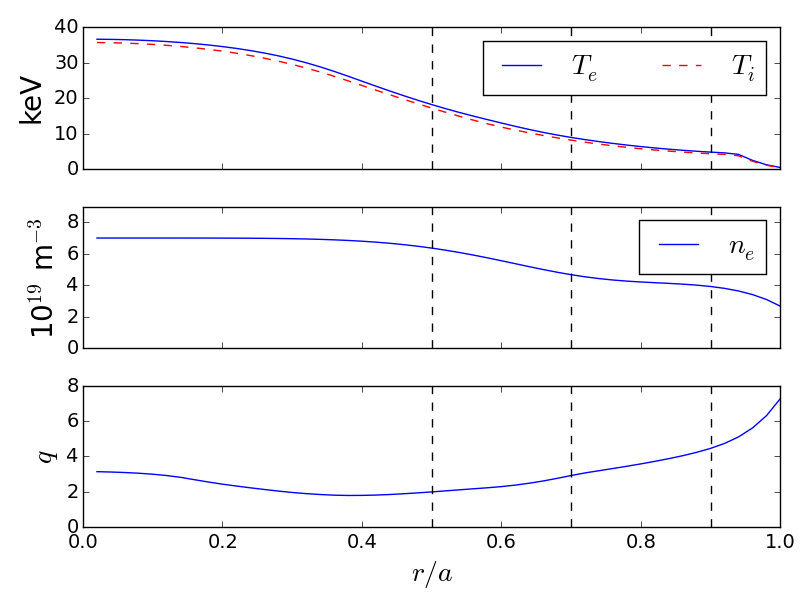
\includegraphics[width=0.7\textwidth]{profiles.png}
\caption{\label{fig:profiles} Radial profiles of temperature, density, and safety factor for the ITER steady state scenario.\cite{Poli2014} Black dashed lines indicate the radial locations that will be considered for neoclassical calculations.}
\end{figure}

We consider an advanced ITER steady state scenario with significant bootstrap current and reversed magnetic shear.\cite{Poli2014} The input power includes 33 MW NBI, 20 MW electron cyclotron (EC), and 20 MW lower hybrid (LH) heating for a fusion gain of $Q = 5$ and toroidal current of 9 MA. The discharge was simulated using the Tokamak Simulation Code (TSC) \cite{Jardin1986} and TRANSP \cite{Hawryluk1980} using a Coppi-Tang \cite{Jardin1993} transport model and EPED1 \cite{Snyder2011} pedestal modeling. The density, temperature, and safety factor $q$ profiles are shown in figure \ref{fig:profiles}. For neoclassical calculations we consider a three species plasma (D, T, and electrons), and we assume that $n_D = n_T = n_e/2$. Neoclassical transport will be analyzed in detail at the radial locations indicated by dashed horizontal lines ($r/a = 0.5, 0.7, 0.9$). Throughout we will use the radial coordinate $r/a \propto \sqrt{\Psi_{\text{T}}}$ where $\Psi_{\text{T}}$ is the toroidal flux.

\FloatBarrier

\section{Free Boundary Equilibrium Calculations and Ripple Magnitude} \label{vmec}

The magnetic equilibrium was computed using the density, temperature, and $q$ profiles from TRANSP along with filamentary models of the toroidal field (TF), poloidal field (PF), and center stack (CS) coils and their corresponding currents. The vacuum fields produced by the three TBMs and the FIs have been modeled using FEMAG.\cite{Shinohara2009} The VMEC free-boundary equilibrium \cite{Hirshman1986} is computed for four geometries: (i) including only the TF ripple, (ii) including TF ripple, TBMs, and FIs, (iii) TF ripple and FIs, and (iv) axisymmetric geometry.  

We define the magnitude of the magnetic field ripple to be,
\begin{gather}
\delta_B = (B_{\text{max}}-B_{\text{min}})/(B_{\text{max}} + B_{\text{min}}), 
\end{gather}
where the maximum and minimum is evaluated at fixed radius and poloidal angle $\theta$. In figure \ref{fig:ripplecontour}, $\delta_B$ is plotted on the poloidal plane for the three rippled VMEC equilibria. The component of $\bm{B}$ with torodial mode number $n = 18$ was removed from the geometry with TBMs and FIs in order to demonstrate the magnitude of the ripple produced by the TBMs alone (bottom right). When only TF ripple is present, significant ripple persists over the entire outboard side, while in the configurations with FIs the ripple is much more localized in $\theta$. When TBMs are present, the ripple is higher in magnitude near the outboard midplane ($\delta_B \approx 1.4\%$), while in the other magnetic configurations $\delta_B \approx$ 1\% near the outboard midplane. For comparison, the TF ripple during standard operations is $0.08\%$ in JET \cite{DeVries2008} and $0.6\%$ in ASDEX Upgrade.\cite{Martitsch2016} 

In figure \ref{fig:toroidalripple}, the magnitude of $\bm{B}$ is plotted as a function of toroidal angle $\zeta$ at $\theta = 0$ and $\theta = \pi/4$. Away from the midplane ($\theta = \pi/4$) the ferritic inserts greatly decrease the magnitude of the TF ripple. Near the midplane the FIs do not decrease the magnitude of the toroidal ripple as strongly, as the number of steel plates is reduced near the midplane.\cite{Shinohara2009} The TBMs add an additional perturbation around $\theta = 0$, as the TBM ports will be located about the midplane. 

\FloatBarrier

\begin{figure}[h!]
\centering
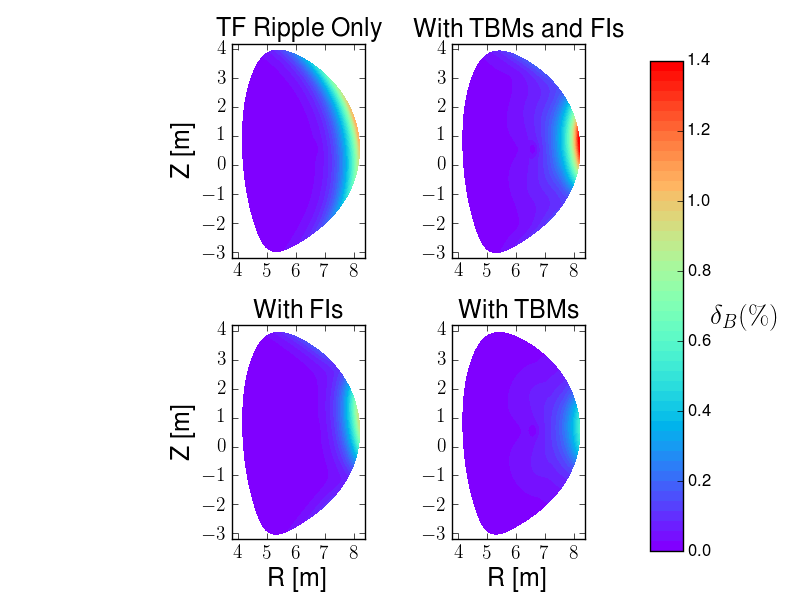
\includegraphics[width=0.7\textwidth]{ripplecontour.png}
\caption{\label{fig:ripplecontour} Magnetic field ripple, $\delta_B = (B_{\text{max}}-B_{\text{min}})/(B_{\text{max}} + B_{\text{min}})$, is plotted on the poloidal plane for VMEC free boundary equilibria including (i) only TF ripple (top left), (ii) TF ripple, TBMs, and FIs (top right), (iii) TF ripple and FIs (bottom left), and (iv) with TBMs only (bottom right). FIs decrease the poloidal extent of the ripple, while TBMs add an additional ripple near the outboard midplane.}
\end{figure}

\begin{figure}[h!]
\centering
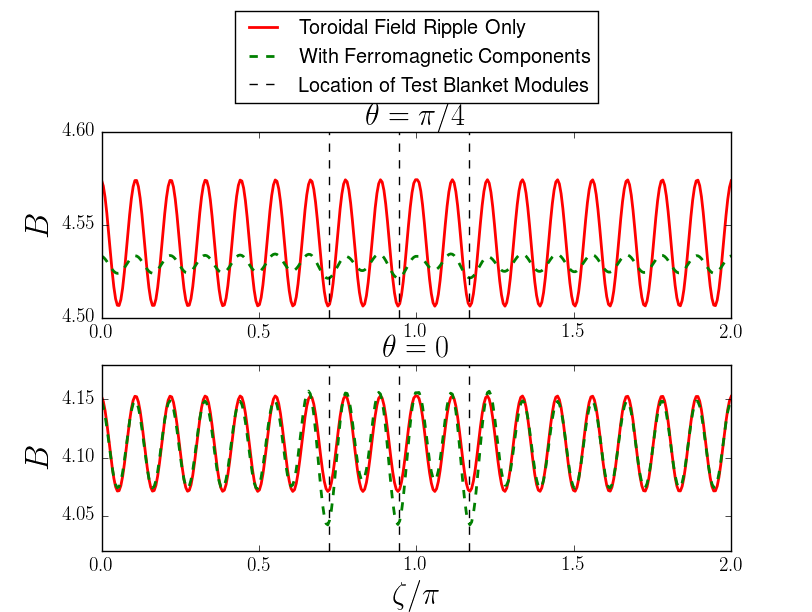
\includegraphics[width=0.7\textwidth]{toroidalripple.png}
\caption{\label{fig:toroidalripple} The magnitude of $\bm{B}$ as a function of toroidal angle ($\zeta$) at $r/a = 1$, $\theta = 0$ and $\pi/4$. Vertical dashed lines indicate the toroidal locations of the TBM ports. The mitigating effect of the FIs is stronger away from the midplane, where an increased number of steel plates are inserted. The TBMs add an additional ripple near their locations at the $\theta = 0$. }
\end{figure}

\FloatBarrier

\section{Estimating Toroidal Rotation}\label{rotation}

In order to predict the ripple transport in ITER, the radial electric field, $E_r = - \Phi'(r) $, must be estimated, as particle and heat fluxes are nonlinear functions of $E_r$. This is equivalent to predicting the parallel flow velocity, $V_{||}$, which scales monotonically with $E_r$.  As we simply wish to determine a plausible value of $E_r$, the difference between $V_{||}$ and $V_{\zeta}$, the toroidal flow, will be unimportant for our estimates. In our calculation of $V_{\zeta}$ the neoclassical torque is ignored. Instead $E_r$ is viewed as an input to neoclassical calculations from which the NTV torque can be obtained. 

For this rotation calculation, angular momentum transport due to neutral beams and turbulence will be considered. There will be an additional torque caused by the radial current of orbit-lost alphas,\cite{Rosenbluth1996} but it will be negligible ($\approx 0.006$ Nm/m$^3$). The following time-independent momentum balance equation is considered in determining $V_{\zeta}$,
\begin{gather}
\nabla \cdot \Pi_{\zeta}^{\text{turb}}(V_{\zeta}) + \nabla \cdot \Pi_{\zeta}^{\text{NC}}(V_{\zeta}) = \tau^{\text{NBI}},
\end{gather}
where $\Pi^{\text{turb}}_{\zeta}$ and $\Pi^{\text{NC}}_{\zeta}$ are the toroidal angular momentum flux densities due to turbulent and neoclassical transport and $\tau^{\text{NBI}}$ is the NBI torque density. For this paper the feedback of $\Pi_{\zeta}^{\text{NC}}$ on $V_{\zeta}$ will not be calculated. Determining the change in rotation due to NTV would require iteratively solving this equation for $V_{\zeta}$, as both $\Pi_{\zeta}^{\text{turb}}$ and $\Pi_{\zeta}^{\text{NC}}$ are functions of $V_{\zeta}$. The quantity $\Pi_{\zeta}^{\text{turb}}$ consists of a diffusive term as well as a term independent of $V_{\zeta}$ which accounts for turbulent intrinsic rotation. An angular momentum pinch will not be considered for this analysis. 
\begin{gather}
\Pi_{\zeta}^{\text{turb}} = -m_i n_i \chi_{\zeta} \langle R \rangle\partder{V_{\zeta}}{r} + \Pi_{\text{int}}
\end{gather}
Here $R$ major radius, $m_i$ is the ion mass, $n_i$ is the ion density, and $\chi_{\zeta}$ is the toroidal angular momentum diffusivity. The flus surface average is denoted by $\langle ... \rangle$,
\begin{gather}
\langle ... \rangle = \frac{1}{V'} \int_0^{2 \pi} d \theta \int_0^{2 \pi} d \zeta \sqrt{g} (...)
\\ V' = \int_0^{2\pi} d \theta \int_0^{2 \pi} d \zeta \sqrt{g},
\end{gather}
where $\sqrt{g}$ is the Jacobian. As it is difficult to model the interactions between external torques and intrinsic rotation, these two effects are considered separately in order to generate two estimates for $V_{\zeta}$. To estimate NBI-drive rotation, TRANSP evolves the rotation profiles by balancing turbulent diffusion (assuming $\chi_{\zeta} = \chi_{i}$, the ion heat diffusivity) and models of neutral beam torques from NUBEAM. The following momentum balance equation is solved,
\begin{gather}
\tau^{\text{NBI}} = -m_i n_i \chi_{i} \langle R \rangle \partder{V_{\zeta}}{r},
\end{gather}
where $\tau^{\text{NBI}}$ is the total beam torque density calculated by NUBEAM including collisional, $\bm{J} \times \bm{B}$, thermalization, and recombination torques.

We consider a semi-analytic intrinsic rotation model to determine the turbulent-driven rotation,\cite{Hillesheim2015}
\begin{gather}
V_{\zeta}(r) = - \langle R \rangle \int_{r}^a \frac{v_{ti} \rho_{*,\theta}} {2 P_r L_T^2} \widetilde{\Pi} (\nu_*) \, d r',
\label{eq:Hillesheim}
\end{gather} 
where $v_{ti} = \sqrt{2T_i/m_i}$ is the ion thermal velocity, $\rho_{*,\theta} = v_{ti} m_i/(e B_{\theta} \langle R \rangle) $ is the poloidal normalized gyroradius, and the Prandtl number $P_r = \chi_{\zeta}/\chi_i$ is taken to be 0.7. The normalized collision frequency $\nu_* = q R v_{ti}/(\nu_{ii} \epsilon^{3/2})$ where $\epsilon = r/\langle R \rangle$ is the inverse aspect ratio and $L_T = - \left( \partial \ln T_i/ \partial r \right)^{-1}$ is the temperature gradient scale length. Equation \ref{eq:Hillesheim} is obtained assuming that $\Pi_{\text{int}}$ balances turbulent momentum diffusion in steady state, $\Pi_{\text{int}} = m_i n_i \chi_{\zeta} \langle R \rangle \partial V_{\zeta}/\partial r$. This model considers the intrinsic torque driven by the neoclassical diamagnetic flows, such that $V_{\zeta} \sim \rho_{*,\theta} v_{ti}$ and $(V_{\zeta}/\langle R \rangle) \Pi_{\text{int}}/Q \sim \rho_{*, \theta}$. It is also assumed that $V_{\zeta} = 0$ at the wall. %Provide justification for these assumptions?? 
The quantity $\widetilde{\Pi} (\nu_*)$ is an order unity function which characterizes the collisionality dependence of rotation reversals, determined from gyrokinetic turbulence simulations,\cite{Barnes2013}
\begin{gather}
\widetilde{\Pi} (\nu_*) = \frac{(\nu_*/\nu_c -1)}{1 + (\nu_*/\nu_c)},
\end{gather}
where $\nu_c = 1.7$. Because of the ITER's low collisionality, we do not expect a rotation reversal, which is correlated with transitioning between the banana and plateau regimes. Equation \ref{eq:Hillesheim} was integrated using profiles for the ITER steady state scenario. 

The rotation predicted by these models is shown in figure \ref{fig:rotation_estimate}. NBI torque contributes to significant rotation at $r/a \lesssim 0.4$ where the torque density also peaks (see figure \ref{fig:alltorque}), while turbulent torque produces much rotation in the pedestal due to the $L_T^{-2}$ scaling of our model.  The intrinsic rotation calculated is comparable to that predicted from theoretical scaling arguments by Parra,\cite{Parra2012} $V_{\zeta} \approx 100$ km/s. At the radii that will be considered for neoclassical calculations (indicated by dashed vertical lines), intrinsic turbulent rotation may dominate over that due to NBI. However, we emphasize that is is an estimate based on scaling arguments, as much uncertainty is inherent in predicting turbulent rotation. 

\FloatBarrier

\begin{figure}[h!]
\centering
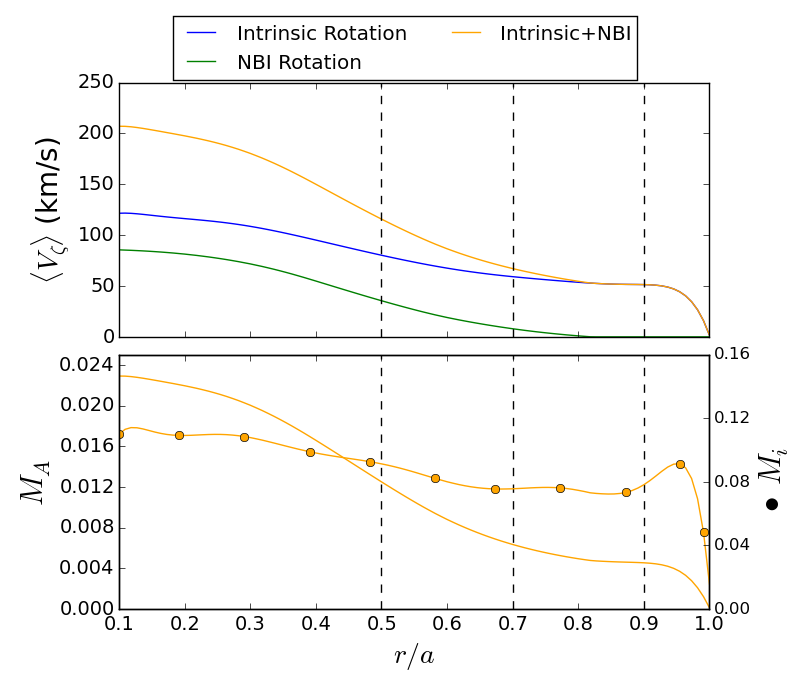
\includegraphics[width=0.7\textwidth]{rotationestimate.png}
\caption{\label{fig:rotation_estimate} Toroidal rotation $V_{\zeta}$ due to turbulence and NBI (top) is shown along with  corresponding Alfv\`{e}n Mach number (bottom, solid), and ion sonic Mach number (bottom, bulleted). The intrinsic rotation calculation uses a semi-analytic model of turbulent momentum redistribution.\cite{Hillesheim2015} The NBI rotation is calculated from turbulent diffusion of NBI torque using NUBEAM and TRANSP.\cite{Poli2014} Dashed vertical lines indicate the radial positions where SFINCS calculations are performed. }
\end{figure}

For stabilization of the resistive wall mode (RWM) in ITER, it has been estimated that a critical central rotation frequency $\omega_0 = V_{\zeta}(0)/\langle R \rangle \gtrsim 5\%$ of the Alfv\`{e}n frequency, $\omega_A = B/(\langle R\rangle\sqrt{\mu_0 \rho_i})$, must be achieved given a peaked rotation profile.\cite{Liu2004} With a central rotation of $\omega_0 \approx 2\% \, M_A$ in figure \ref{fig:rotation_estimate}, it may be difficult to suppress the RWM in ITER with rotation alone. As this calculation does not take into account magnetic braking, $\omega_0/\omega_A$ is likely to be smaller than what is shown. Additionally, the TBM are known to increase the critical rotation frequency as they have a much shorter resistive time scale than the wall.\cite{Liu2004} More recent analysis has shown that even above such a critical rotation value, the plasma can become unstable due to resonances between the drift frequency and bounce frequency.\cite{Berkery2010, Liu2009}

\FloatBarrier

\section{Relationship Between $E_r$ and $V_{||}$}\label{Erandv}

Equipped with a profile of $V_{\zeta}$, neoclassical calculations of $V_{||}$ are made in order to determine the radial electric field. The parallel flow velocity for species $a$ is computed from the neoclassical distribution function,
\begin{gather}
V^a_{||} = \left(\frac{1}{n_a}\right) \int d^3 v \, v_{||} f_a,
\label{eq:parallelflow}
\end{gather}
which we calculate with the Stellarator Fokker-Planck Iterative Neoclassical Conservative Solver (SFINCS) \cite{Landreman2014} code.
SFINCS is used to solve a radially-local drift kinetic equation for the gyro-averaged distribution function, $f_{a1}$, on a single flux surface including coupling between species. 
\begin{gather}
( v_{||} \bm{b} + \bm{v}_E + \bm{v}_{\text{m}a}) \cdot (\nabla f_{a1})  - C(f_{a1}) = - \bm{v}_{\text{m}a} \cdot \nabla \psi \left( \partder{f_{a0}}{\psi} \right) + \frac{Z_a e v_{||} B \langle E_{||} B \rangle}{T_a \langle B^2 \rangle } f_{a0}.
\label{kineticequation}
\end{gather} 
\hspace{-1mm}
Here $a$ indicates species, $f_{a0}$ is an equilibrium Maxwellian, $\psi = \Psi_{\text{T}}/2\pi$, and $C$ is a linearized Fokker-Planck collision operator. The $\bm{E} \times \bm{B}$ drift is 
\begin{gather}
\bm{v}_E = \frac{1}{B^2} \bm{B} \times \nabla \Phi
\end{gather} 
and the radial magnetic drift is
\begin{gather}
\bm{v}_{\text{m}a} \cdot \nabla \psi = \frac{1}{2\Omega_a B} \left(v_{||}^2 + \frac{v_{\perp}^2}{2} \right) \bm{b} \times \nabla B \cdot \nabla \psi,
\label{magneticdrift}
\end{gather} 
where $v_{||}$ and $v_{\perp}$ are the components of the velocity coordinate parallel and perpendicular to $\bm{b}$, respectively. The quantity $\Omega_a = Z_aeB^2/m_a$ is the gyrofrequency. Transport quantities have been calculated using the steady state scenario ion and electron profiles and VMEC geometry. The second term on the right hand side of eq. \ref{kineticequation} proportional to $E_{||}$ is negligible for this non-inductive scenario with loop voltage $ \approx 10^{-4}$ V. For the calculations presented sections \ref{Erandv}, \ref{torque}, \ref{scaling}, and \ref{heatflux}, $\bm{v}_{\text{m}a} \cdot \nabla f_{a1}$ is dropped. The effect of keeping this term is shown to be small in section \ref{mds}.

The relationship between $E_r$ and $V_{||}$ for electrons and ions at $r/a = 0.9$ is shown in figure \ref{fig:Er_flow}. Note that only one curve is shown for each species as the addition of ripple fields did not change the dependence of $V_{||}$ on $E_r$ significantly ($\leq 5 \%$). While radial transport of heat and particles changes significantly in the presence of small ripple fields (see sections \ref{torque}, \ref{scaling}, and \ref{heatflux}), the parallel flow is much less sensitive to the perturbing field. It can be shown (see appendix \ref{parallelflow}) that the component of $f_1$ that contributes to $V_{||}$ is of higher order in $\nu_* \ll 1 $ than the component that contributes to $\Gamma_{\psi}$. 

\begin{figure}[h!]
\centering
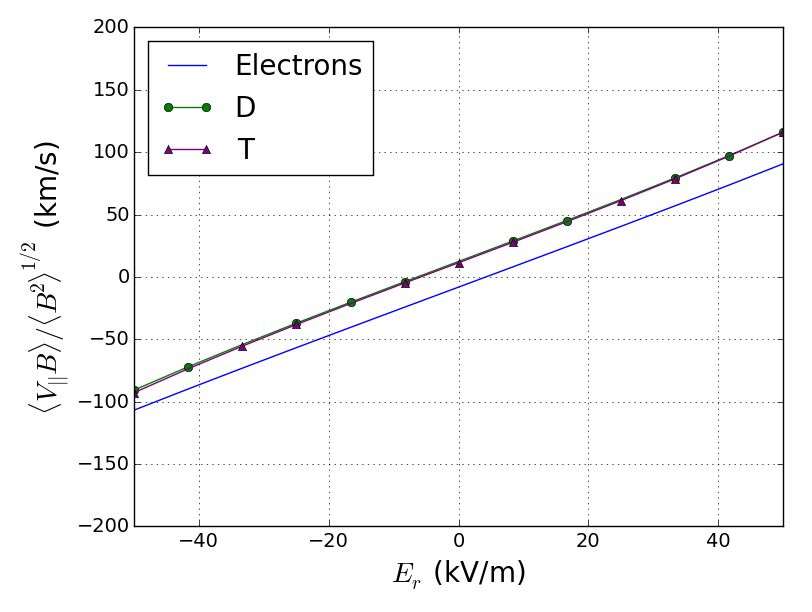
\includegraphics[width=.7\textwidth]{Er_flow.png}
\caption{\label{fig:Er_flow} SFINCS calculation of the parallel flow $V_{||}$ at $r/a = 0.9$ for ions and electrons. The addition of ripple does not change tokamak neoclassical relationship between $E_r$ and $V_{||}$ by a discernible amount on this scale although the radial particle fluxes, $\Gamma_{\psi}$, are sensitive to perturbing field.}
\end{figure}

\FloatBarrier

\section{Torque Calculation}\label{torque}

The NTV torque density, $\tau^{\text{NTV}}$, is calculated from radial particle fluxes, $\Gamma_{\psi}$, 
\begin{gather}
\Gamma_{\psi,a} = \left \langle \int d^3v (\bm{v}_{\text{m}a} \cdot \nabla \psi) f_a \right \rangle,
\label{eq:particleflux}
\end{gather}
using the flux-friction relation,
\begin{gather}
\tau^{\text{NTV}} = - B^{\theta} \sum_a n_a q_a \Gamma_{\psi, a},
\end{gather}
where $B^{\theta} = \bm{B} \cdot \nabla \theta$ and the summation is performed over species. This expression relates radial particle transport to a toroidal angular momentum source caused by the non-axisymmetric field. This relationship can be derived from action-angle coordinates,\cite{Albert2016} neoclassical moment equations,\cite{Shaing1986} and from the definition of the drift-driven flux.\cite{Shaing2006} 

The calculation of $\tau^{\text{NTV}}$ for three geometries at $r/a = 0.9$ is shown in figure \ref{fig:Torque_ErandV}. The axisymmetric geometry does not contribute to NTV torque, as expected. Overall, the magnitude of the torque density with only TF ripple is larger than that with the addition of both the FIs and the TBMs.  In figure \ref{fig:Torque_comparingTBMandFI} we show that the TBMs produce much less torque than the $n = 18$ component of $\bm{B}$, so the decrease in torque magnitude with FIs and TBMs can be attributed to the decrease in ripple in the presence of FIs. The dashed vertical line indicates the value of $V_{||}$ and $E_r$ predicted from the intrinsic rotation model, and the dash-dot vertical line indicates that of the NBI rotation model. At both estimates of rotation, the presence of ferritic components decreases the magnitude of the torque density by $\approx 75\%$. The circle indicates the offset rotation at the ambipolar $E_r$. If no other angular momentum source were present in the system, the NTV torque would drive the plasma to rotate at this velocity. Although $\tau^{\text{NTV}}$ differ significantly between the two geometries they have similar offset rotation velocities, $V_{\zeta}$ = -10 km/s with TF ripple only and -6 km/s with TBMs and FIs. Note that for $E_r$ greater than this ambipolar value, $\tau^{\text{NTV}}$ is counter-current while neutral beams and turbulence drive rotation in the co-current direction, so $\tau^{\text{NTV}}$ is a damping torque. 

The NTV torque due to TF ripple only is larger in magnitude than $\tau^{\text{NBI}}$ while that with TBMs and FIs is of similar magnitude (see figure \ref{fig:alltorque}). NTV may also compete with the turbulent torque, $\tau^{\text{turb}} = - \nabla \cdot \Pi_{\text{int}} \approx 0.1$ Nm/m$^3$ at this radius. Therefore, NTV torque may be key in determining the edge rotation in ITER. Note that the magnitude of $\tau^{\text{NTV}}$ peaks near $E_r = 0$ where $1/\nu$ transport dominates. While this region is avoided at this radius, $1/\nu$ transport may become significant at smaller radii, as will be discussed below. 

\FloatBarrier

\begin{figure}[h!]
\centering
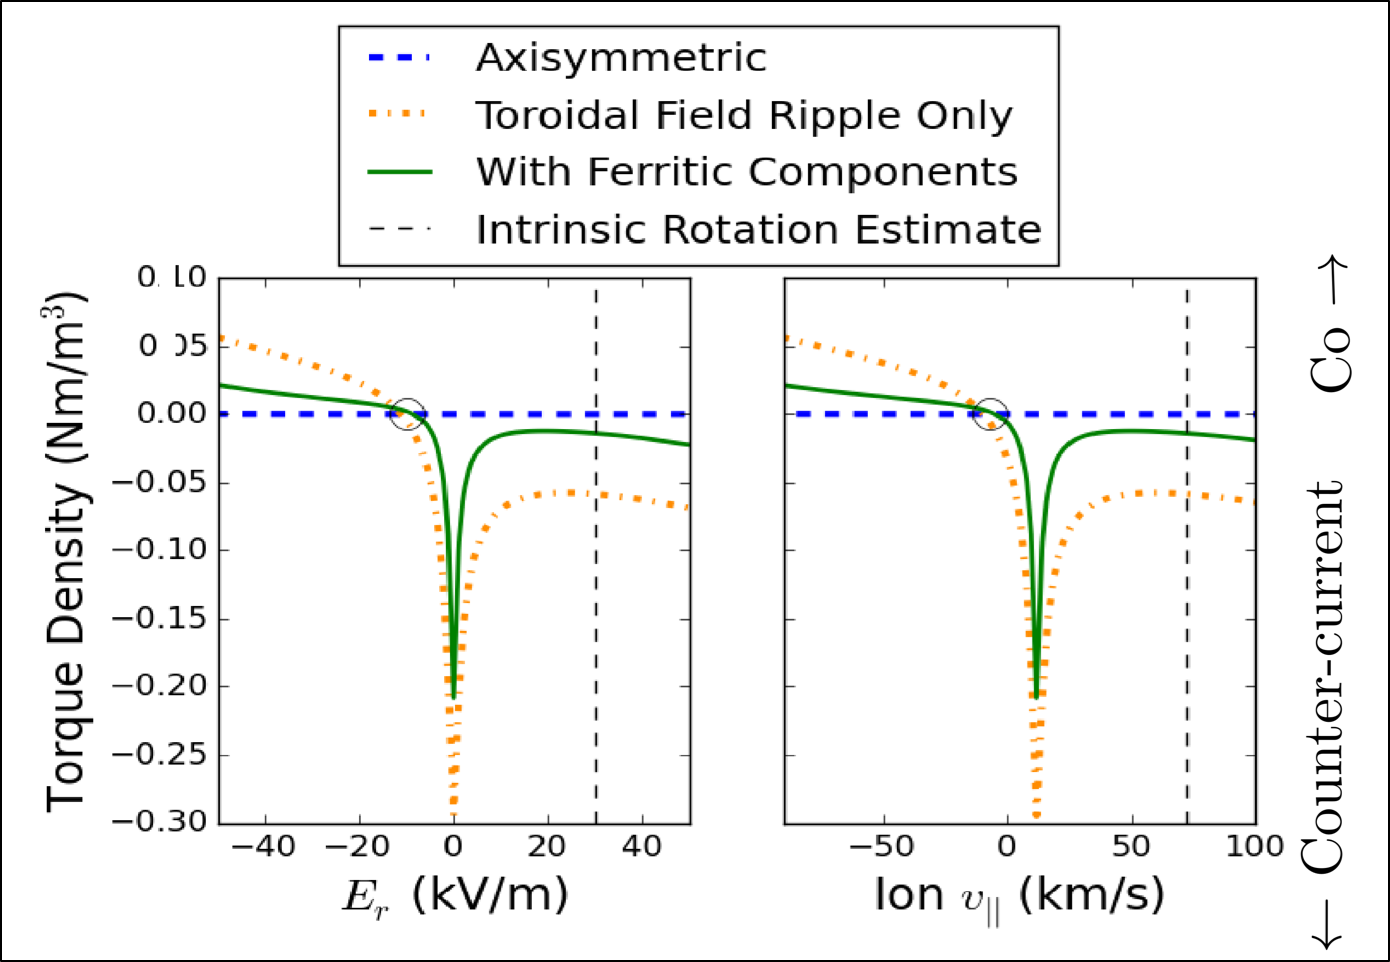
\includegraphics[width=0.7\textwidth]{Torque_ErandV.png}
\caption{\label{fig:Torque_ErandV} SFINCS calculation of NTV torque density as a function of $E_r$ and $V_{||}$ at $r/a = 0.9$ is shown for 3 VMEC geometries: (i) axisymmettic (blue dashed), (ii) with TF ripple only (orange dash-dot), and (iii) TF ripple with FIs and TBMs (green solid). The vertical dashed line indicates the estimate of $E_r$ and $V_{||}$ based on the intrinsic rotation model, and the dash-dot line indicates that predicted by the NBI rotation model. The circle denotes the offset rotation at $V_{||} \sim -10$ km/s. The magnitude of $\tau^{\text{NTV}}$ at this radius is of similar magnitude to the NBI and turbulent torques but is opposite in direction (see figure \ref{fig:alltorque}).}
\end{figure}

In order to decouple the influence of the FI ripple and the TBM ripple, the torque density is calculated at $r/a = 0.9$ for geometries including (i) TF ripple with FIs and TBMs, (ii) TF ripple with FIs, and (iii) only TBMs, shown in figure \ref{fig:Torque_comparingTBMandFI}. The same VMEC geometry is used for each of these NTV calculations, but the $n =18$ ripple is used in the FI only case while the other Fourier modes are included in the TBM only case. As SFINCS is not linearized in the perturbing field, the torque due to both FIs and TBMs is not the sum of the torques due to these ripple fields considered individually. The $n = 18$ component drives about 100 times more torque than the other Fourier components of $\bm{B}$.  While the FIs decrease the magnitude of the $n =18$ component of $B$, the TBM contributes to low mode numbers (mostly $n = 1$). In the $\sqrt{\nu}$ regime ion transport scales as $\Gamma_{\psi} \sim \sqrt{n}$ and in the $1/\nu$ regime $\Gamma_{\psi} \sim n^2$,\cite{Shaing2010} so it is reasonable to expect that the higher harmonic ripple of the FIs would drive more torque. Moreover, from simple diffusive transport scaling we can see that decreasing the extent of the ripple will decrease neoclassical transport. When transport is dominated by the $\bm{E} \times \bm{B}$ precession frequency $\omega_E = E_r/B$, if the poloidal extent of the ripple, $\Delta \theta$, is decreased, the characteristic time scale for detrapping, $\Delta t \sim \Delta \theta/ \omega_E$, will decrease. If the characteristic diffusion scales as $D \sim \Delta x^2/\Delta t$, reducing the poloidal extent of ripple will decrease transport. 

\begin{figure}[h!]
\centering
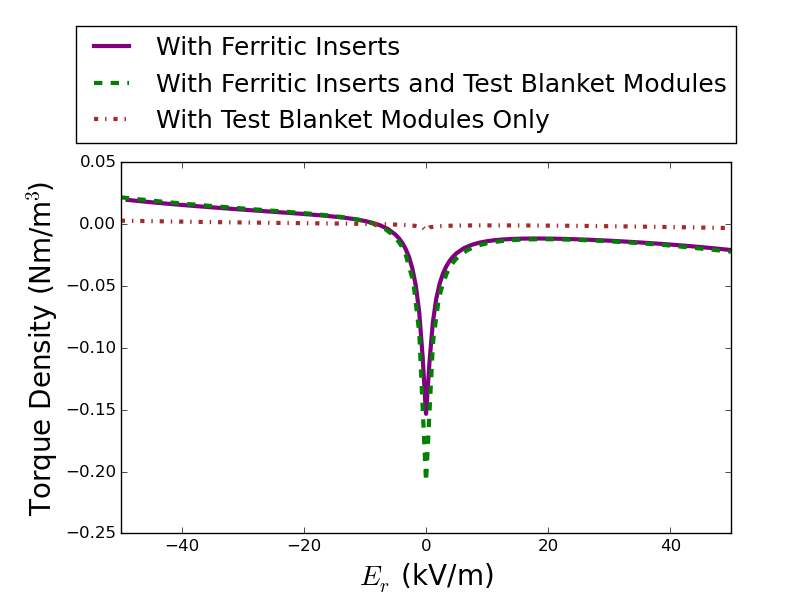
\includegraphics[width=0.7\textwidth]{Torque_comparingTBMandFI.png}
\caption{\label{fig:Torque_comparingTBMandFI} The NTV torque density at $r/a = 0.9$ for three magnetic geometries: (i) with FIs (purple solid), (ii) with TBMs (brown dash dot), and (iii) with FIs and TBMs (green dashed). The low toroidal mode number TBM ripple does not contribute as strongly to the NTV torque density as the $n = 18$ components of $\bm{B}$ do.}
\end{figure}

In figure \ref{fig:Torque_radiusscaling}, the SFINCS calculation of $\tau^{\text{NTV}}$ with TF ripple only is shown at $r/a$ = 0.5, 0.7, and 0.9. For these three radii the maximum $\delta_B = 0.26\%$,  0.51\%, and 0.82\% respectively. It is reasonable to expect that the magnitude of transport decreases with decreasing ripple, as particles fluxes in the $1/\nu$ regime scale as $\Gamma_{\psi} \sim (\delta_B)^2$\cite{Shaing2003} and in the $\sqrt{\nu}$ regime they scale as $ \Gamma_{\psi}\sim (\delta_B)$.\cite{Shaing2008} The $\sqrt{\nu}$ regime applies for $\abs{E_r} \gtrsim 0.2$ kV, where $\omega_E > \nu_{ii}/\epsilon$ and the $1/\nu$ regime applies when $\abs{E_r} \lesssim 0.2$ kV. Moreover, the poloidal extent of the ripple decreases with decreasing radius, so particles spend less time in the rippled region. On the other hand, transport in the $\sqrt{\nu}$ regime also scales with $T_i$, $\Gamma_{\psi} \sim v_{ti}^4 \sqrt{\nu_{ii}} \sim T_i^{5/4}$. The combined effect of decreased ripple and increased temperature with decreasing radius leads to comparable torques with decreasing radius in the $\sqrt{\nu}$ regime. The scaling with $T_i$ is even stronger in the $1/\nu$ regime, where $\Gamma_{\psi} \sim v_{ti}^4/\nu_{ii} \sim T^{7/2}$. Indeed, we find that the magnitude of $\tau^{\text{NTV}}$ at $E_r = 0$ increases with decreasing radius. 

\begin{figure}[h!]
\centering
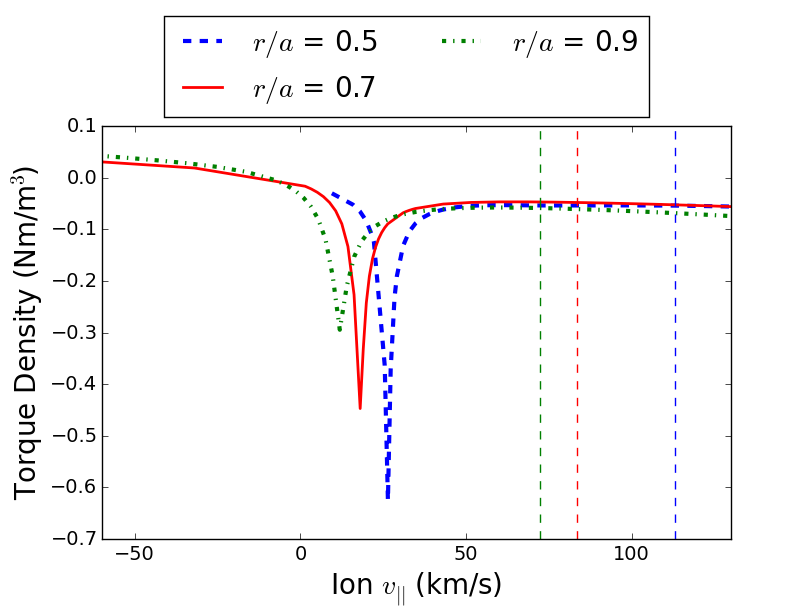
\includegraphics[width=0.7\textwidth]
{Torque_radiusscaling.png}
\caption{\label{fig:Torque_radiusscaling} SFINCS calculation of NTV torque density ($\tau^{\text{NTV}}$) as a function of ion $V_{||}$ for VMEC geometry with TF ripple only at $r/a$ = 0.5 (blue solid), 0.7 (red dashed), and 0.9 (green dash-dot). Although the field ripple decreases with radius (maximum $\delta_B = 0.82\%$ at $r/a = 0.9$, $\delta_B = 0.51\%$ at $r/a = 0.7$, $\delta_B = 0.26\%$ at $r/a = 0.5$), transport near $E_r = 0$ increases with decreasing radius because of strong scaling of neoclassical transport with temperature in the $1/\nu$ regime.\cite{Shaing2003}}
\end{figure}

In figure \ref{fig:alltorque}, we compare the magnitude of $\tau^{\text{NTV}}$ with $\tau^{\text{NBI}}$ and $\tau^{\text{turb}} = -\nabla \cdot \Pi_{\text{int}}$, the turbulent momentum source causing intrinsic rotation. For the $\tau^{\text{NTV}}$ profile, the intrinsic rotation model and NBI rotation model are used to estimate $E_r$ at each radius. At $r/a = 0.55$, $\tau^{\text{NTV}}$ with the NBI rotation model ($E_r$ = 0.03 kV/m) is about 20 times larger than $\tau^{\text{NTV}}$ with the intrinsic rotation model ($E_r$ = 46.9 kV/m), as the $E_r$ predicted by the NBI model is small enough that $1/\nu$ transport may dominate. The quantity $\tau^{\text{NBI}}$ is determined from NUBEAM calculations,\cite{Poli2014} and $\tau^{\text{turb}}$ is estimated using $\Pi_{\text{int}} \sim (\rho_{\theta}/L_T) \widetilde{\Pi}(\nu_*) Q (\langle R \rangle/v_{ti})$ (see appendix \ref{turbQ}). Note that the turbulent torque produces much rotation in the pedestal according to this model as $\tau^{\text{turb}} \propto 1/L_T$. The integrated NTV torque with the turbulent rotation model, -40 Nm, is comparable to the NBI torque, 35 Nm, while the turbulent torque is significantly larger, 93 Nm. The integrated NTV torque with the NBI rotation model is -57 Nm.

Near the edge ($0.5 \lesssim r/a \lesssim 0.9$), NTV torque may dominate the rotation profile and will likely significantly damp rotation, decreasing MHD stability. However, the resulting rotation profile may be sheared because of the significant counter-current NTV source at the edge and co-current NBI source in the core. This may provide a rotation shear as high as $\Delta V_{\zeta}/ \Delta r \approx 0.8 (v_{ti}/R)$ near $r_N = 0.5$, possibly large enough to suppress microturbulence\cite{Hahm1994} and promote the formation of an internal transport barrier. The rotation shear may be even more significant if the rotation profile is similar to that predicted by the NBI rotation model because of the magnified $\tau^{NTV}$ near $r_N = 0.55$. 

\begin{figure}[h!]
\centering
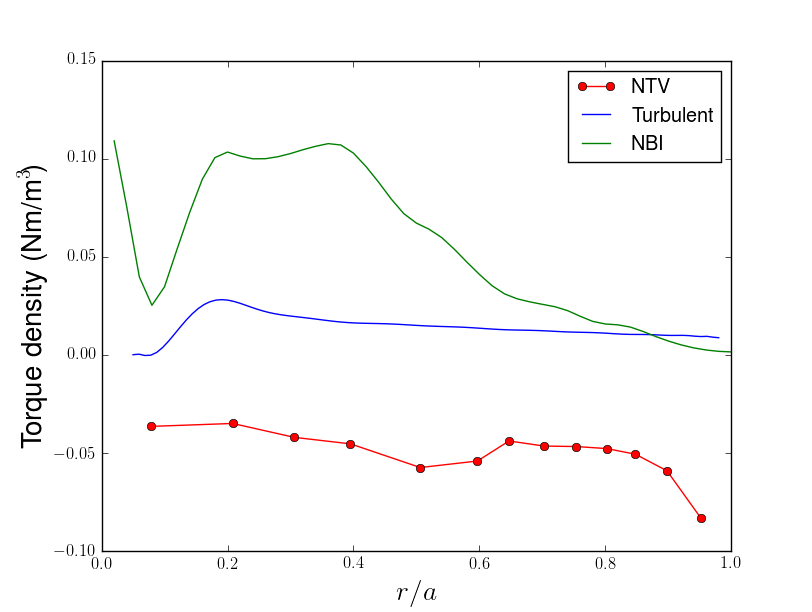
\includegraphics[width=0.7\textwidth]{AllTorquePlot.png}
\caption{\label{fig:alltorque} Torque density profiles of NTV torque density ($\tau^{\text{NTV}}$) calculated with SFINCS, NBI torque density calculated from NUBEAM ($\tau^{\text{NBI}}$), and estimate of turbulent intrinsic rotation momentum source ($\tau^{\text{turb}}$). The quantity $\tau^{\text{NTV}}$ is calculated using $E_r$ determined by the intrinsic rotation model and NBI rotation model described in section \ref{rotation}. Turbulent torque is estimated using $\tau^{\text{turb}} \sim -\Pi_{\text{int}}/a$ where $\Pi_{\text{int}} \sim \rho_{*, \theta} \widetilde{\Pi}(\nu_*) Q \langle R \rangle/v_{ti}$ (see appendix \ref{turbQ} for details).}
\end{figure}

\FloatBarrier

\section{Scaling with Ripple Magnitude}\label{scaling}
The scaling of NTV transport with the magnitude of $\delta_B$ shows some agreement with that predicted by Shaing for the $\sqrt{\nu}$ and $\nu$ regimes.\cite{Shaing2008, Shaing2009} In figure \ref{fig:scalescan}, the NTV torque density calculated by SFINCS is shown as a function of the magnitude of the ripple, $\delta_B$, for TF only geometry. The additional ferromagnetic ripple is not included, while the $n= 18$ component of $\bm{B}$ is rescaled. The quantity $\tau^{\text{NTV}}$ is calculated at $r/a = 0.9$ with $E_r = 30$ kV/m, corresponding to the intrinsic rotation estimate. The color-shaded background indicates the approximate regions of applicability of the $\sqrt{\nu}$ and $\nu$ regimes. The $1/\nu$ regime does not apply at this $E_r$, as $\omega_E \gg \nu/\epsilon$.\cite{Shaing2003} The radial electric field is also large enough that the resonance between $\bm{v}_{E}$ and $\bm{v}_{\text{m}}$ cannot occur, so the superbanana plateau \cite{Shaing2009_sbp} and superbanana \cite{Shaing2009_sb} regimes are avoided. 

In the collisional boundary layer, neoclassical fluxes scale as $\sqrt{\nu}$.\cite{Shaing2008} This regime becomes relevant when the poloidal $\bm{E} \times \bm{B}$ precession frequency is larger than the effective collision frequency of detrapping banana particles, $\nu/\epsilon < \omega_E$, and the ripple magnitude is not large enough for collisionless detrapping to take effect, $\delta_B < \left(  \epsilon \nu/\omega_E \right)^{1/2}$. 
In the collisionless trapping-retrapping regime, neoclassical fluxes scale with $\nu$.\cite{Shaing2009} This regime becomes relevant when $\delta_B > \left(  \epsilon \nu/\omega_E \right)^{1/2}$ and the perturbing field becomes large enough that poloidally trapped particles can become detrapped and retrapped by the ripple. In the $\sqrt{\nu}$ regime $\tau^{\text{NTV}} \sim \delta_B^2$ and in the $\nu$ regime $\tau^{\text{NTV}} \sim \delta_B$. For $\delta_B$ smaller than $\delta_B^* = 0.82\%$, the actual value of ripple at $r/a=0.9$ for ITER geometry, the scaling of $\tau^{\text{NTV}}$ with $\delta_B$ is slightly shallower than what is predicted. 
As $\delta_B$ nears the boundary between the $\sqrt{\nu}$ and $\nu$ regimes in figure \ref{fig:scalescan}, the scaling of $\tau^{\text{NTV}}$ with $\delta_B$ becomes even less stiff and shows some agreement within the $\sqrt{\nu}$ regime. When $\delta_B \sim \epsilon$, the poloidal field variation no longer becomes the dominant perturbation, so perturbations this large have not been considered. The departure of numerical results from predicted scaling can be attributed to the analytic models which use a bounce-averaged kinetic equation and assume large aspect ratio. 

\begin{figure}[h!]
\centering
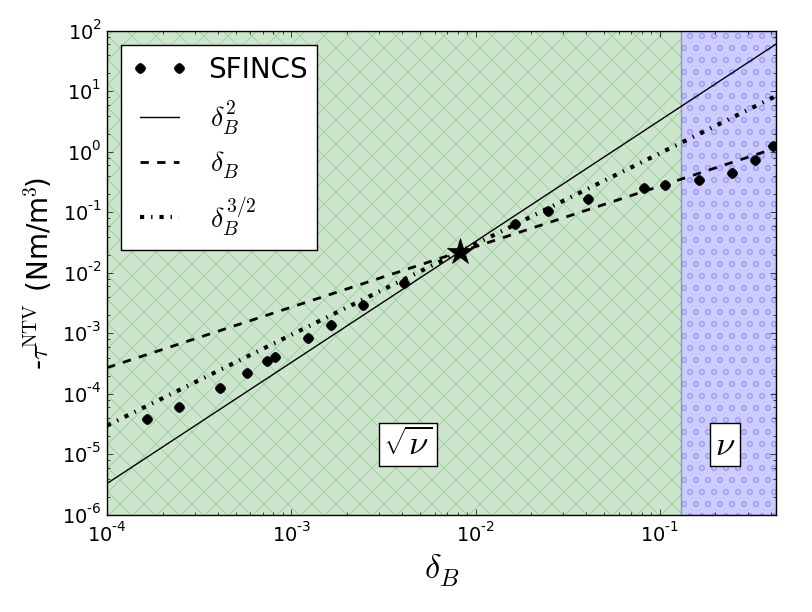
\includegraphics[width=0.7\textwidth]
{scalescan.png}
\caption{\label{fig:scalescan} SFINCS calculations of NTV torque density as a function of $\delta_B$ at $r/a = 0.9$. A single value of $E_r = 30$ kV/m is used corresponding to the intrinsic rotation estimate. Color-shaded area indicates the approximate regions of applicability for rippled tokamak regimes described by Shaing: the $\sqrt{\nu}$ regime where $\tau^{\text{NTV}} \sim \delta_B^2$\cite{Shaing2008} and the $\nu$ regime where $\tau^{\text{NTV}} \sim \delta_B$.\cite{Shaing2009} }
\end{figure} 

\FloatBarrier

\section{Heat Flux Calculation}\label{heatflux}
As well as driving non-ambipolar particle fluxes, the breaking of toroidal symmetry drives an additional neoclassical heat flux. In figure \ref{fig:HeatFlux}, the SFINCS calculation of heat flux is shown for three magnetic geometries: (i) axisymmetric (blue solid), (ii) with TF ripple only (green dashed), and (iii) TF ripple with TBMs and FIs (red dash-dot). In the presence of TF ripple, the ripple drives an additional heat flux that is comparable to the axisymmetric heat flux. However, with the addition of the FIs the heat flux is reduced to the magnitude of the axisymmetric value, except near $E_r = 0$ where $1/\nu$ transport dominates. 

While the radial ripple-drive particle fluxes will significantly alter the ITER angular momentum transport, the neoclassical heat fluxes are insignificant in comparison to the turbulent heat flux. Note that the neoclassical heat flux is $\lesssim 5\%$  of the heat flux calculated from heating and fusion rate profiles (see appendix \ref{turbQ}), $Q\approx 0.2$ MW/m$^2$. Thus we can attribute $\gtrsim 95\%$ of the heat transport to turbulence. If ITER ripple were scaled up to $\delta_B \gtrsim 30\%$, the neoclassical ripple heat transport would be comparable to the anomalous transport.

\begin{figure}[h!]
\centering
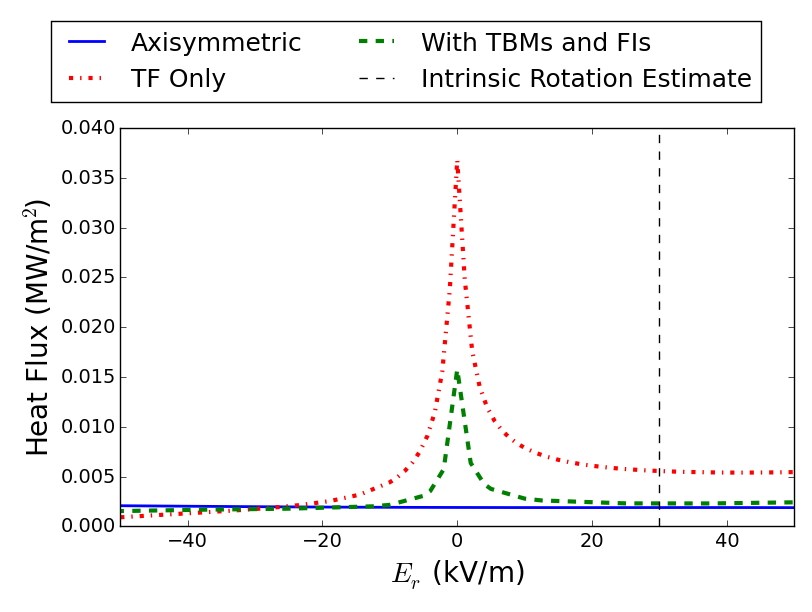
\includegraphics[width=0.7\textwidth]
{HeatFlux.png}
\caption{\label{fig:HeatFlux} SFINCS calculation of neoclassical heat flux at $r/a = 0.9$ for three magnetic geometries: (i) axisymmetric (blue solid), (ii) with TF ripple only (green dashed), and (iii) TF ripple with TBMs and FIs (red dash-dot). The vertical dashed line corresponds to the intrinsic rotation $E_r$ estiamte, and the dash-dot line corresponds to the NBI rotation $E_r$ estimate. These heat fluxes are much smaller than the anomalous heat transport is likely to be, $Q\approx 0.2$ MW/m$^2$,}
\end{figure}

\FloatBarrier

\section{Tangential Magnetic Drifts}\label{mds}
Although $(\bm{v}_E + \bm{v}_{\text{m}}) \cdot \nabla f_1$ is formally of lower order than the other terms in eq. \ref{kineticequation}, it has been found to be important when $\rho_* \sim \nu_*$ \cite{Calvo2016, Matsuoka2015} and has been included in other calculations of 3D neoclassical transport. In the SFINCS calculations shown in sections \ref{Erandv}, \ref{torque}, \ref{scaling}, and \ref{heatflux}, $\bm{v}_{\text{m}} \cdot \nabla f_1$ has not been included. As SFINCS does not maintain radial coupling of $f_1$, the poloidal and toroidal drifts are retained in this term while the radial drift is not. Note that the radial magnetic drift is retained in $\bm{v}_{\text{m}} \cdot \nabla f_0$. 

Several issues must be considered when the poloidal and toroidal magnetic drifts are present. A coordinate-dependence can be introduced when the $\bm{v}_{\text{m}} \cdot \nabla \psi$ term is ignored, as $\nabla \theta$ and $\nabla \zeta$ do not necessarily lie on the flux surface. For a coordinate-independent form, one must project $\bm{v}_{\text{m}}$ onto the flux surface. Additionally, when these terms are retained the effective particle trajectories do not satisfy $\dot{\xi} (\xi = \pm 1) = 0$ where $\xi = v_{||}/v$, so a velocity-dependent factor can be included for regularization.  This ensures that particles with $\mu = 0$ conserve $\mu$. It also eliminates the need for additional particle and heat sources due to the radially local assumption and preserves ambipolarity of axisymmetric systems.\cite{Sugama2016} To this end, we employ a coordinate-independent magnetic drift perpendicular to $\nabla \psi$,
\begin{gather}
\bm{v}_{\text{m}a}^{\perp} = \frac{v^2}{2B^2 \Omega_a} (\bm{B} \times \nabla \psi) \left[(1+\xi^2) \frac{\kappa_n \rvert \nabla \psi \rvert}{B} - (1 - \xi^2) \frac{\mu_0}{B} \der{p}{\psi} \right],
\end{gather}
where $\kappa_n = \nabla \psi \cdot (\bm{b} \cdot \nabla \bm{b})/(\rvert \nabla \psi \rvert)$ is the normal curvature. In order to regularize the first term, we multiply it by $\alpha(\xi) = (1-\xi^2)(1+\xi^2)$. This gives
\begin{gather}
\bm{v}_{\text{m}a}^{\perp} = \frac{v^2}{2B^2 \Omega_a} (\bm{B} \times \nabla \psi) (1 - \xi^2) \frac{(\nabla \psi \cdot \nabla B)}{\rvert \nabla \psi \rvert^2}.
\end{gather}
Note that this is similar to the form presented by Sugama,\cite{Sugama2016} except for we have chosen a different form of regularization. We compare this form with the form of magnetic drifts without projection or regularization,
\begin{gather}
\bm{v}_{\text{m}a} = \frac{v^2}{2 \Omega_a B^2} (1 + \xi^2) \bm{B} \times \nabla B + \frac{v^2}{\Omega_a B} \xi^2 \nabla \times \bm{B}.
\end{gather}

An $E_r$ scan at $r/a = 0.7$, where $\rho_*$ becomes comparable to $\nu_*$, is shown in figure \ref{fig:driftschemes}. When $\bm{v}_{\text{m}} \cdot \nabla f_1$ is added to the kinetic equation, the typical peak at $E_r = 0$ is shifted toward a slightly negative $E_r$, corresponding to the region where $\bm{v}_E + \bm{v}_M = 0$. With the projected form of the drifts, $\bm{v}_{\text{m}}^{\perp}$, this peak is much shallower than with the unprojected drift scheme, but otherwise the two schemes predict similar behavior. Overall, the addition of $v_{\text{m}} \cdot \nabla f_1$ has a negligible effect on transport for the large $E_r$ predicted for ITER, and choice of magnetic drift scheme would not dramatically change the results in previous sections.  

\begin{figure}[h!]
\centering
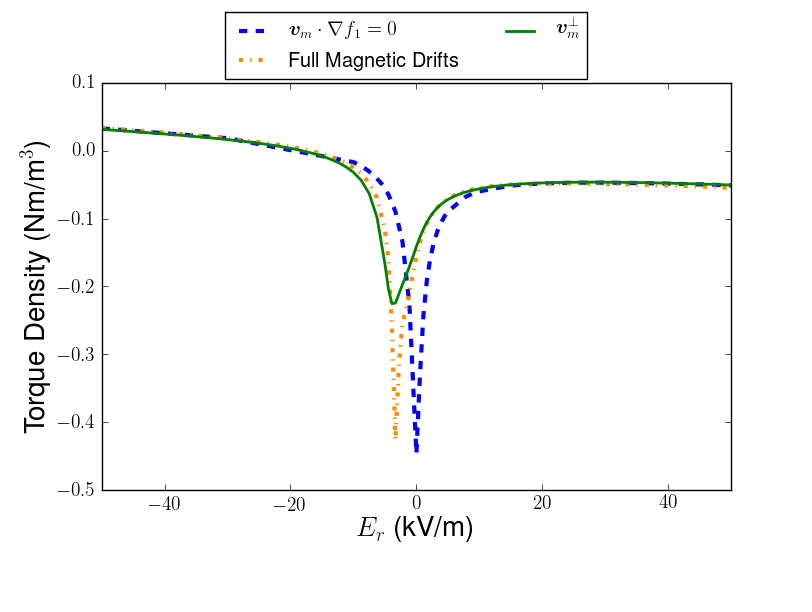
\includegraphics[width=0.7\textwidth]{mdscomparison.png}
\caption{\label{fig:driftschemes} Comparison of magnetic drift models at $r/a = 0.7$. NTV torque density is calculated for the ITER steady state scenario as a function of $E_r$. The addition of $\bm{v}_{\text{m}} \cdot \nabla f_1$ in the kinetic equation solved by SFINCS has little effect on the neoclassical transport at this radius. }
\end{figure}

\FloatBarrier

\section{Summary}\label{summary}

We calculate neoclassical transport in the presence of 3D magnetic fields, including toroidal field ripple and ferromagnetic components, for an ITER steady state scenario. We use an intrinsic turbulent rotation model described to estimate $E_r$ for neoclassical calculations. We find that even without $\tau^{\text{NTV}}$, toroidal rotation will be $\lesssim 2\% \,M_A$, which is likely not large enough to suppress resistive wall modes.\cite{Liu2004} We use VMEC free boundary equilibria in the presence of ripple fields to calculate neoclassical particle and heat fluxes using the drift-kinetic solver, SFINCS. At large radii $r/a \gtrsim 0.5$, $\tau^{\text{NTV}}$ is comparable to $\tau^{\text{NBI}}$ in magnitude but opposite in sign, which may result in flow damping at the edge and a decrease in MHD stability. The integral NTV torque, -40 Nm, is larger in magnitude than NBI torque, 35 Nm, so non-resonant magnetic braking cannot be ignored in analysis of ITER rotation. The torque profile may also result in a significant rotation shear which could suppress turbulent transport. While the addition of FIs significantly reduces the transport ($\approx 80\%$ reduction at $r/a = 0.9$), the TBMs themselves produce very little NTV torque. Further analysis is needed to determine if penetration of the TBM ripple fields will form islands and produce resonant torques. While the NTV torque has been shown to be important for ITER angular momentum balance, iteratively solving for the rotation profile with $\tau^{\text{NTV}}$ will be left for future consideration.

\appendix

\section{Parallel Flow is Less Sensitive to Perturbing Field Than Particle Fluxes} \label{parallelflow}
In this section we will show that the contribution to $V_{||}$ from $f_1$ is of order $\nu_* \ll 1$ smaller than the contribution to $\Gamma_{\psi}$. As $V_{||}$ is an odd moment of $v_{||}$ (eq. \ref{eq:parallelflow}), only the component of $f_1$ that is odd in $v_{||}$ will contribute. Similarly, only the component of $f_1$ that is even in $v_{||}$ will contribute to $\Gamma_{\psi}$ as it is an even moment of $v_{||}$ (eq. \ref{eq:particleflux}). We start with the following drift kinetic equation,
\begin{gather}
v_{||} \bm{b} \cdot \nabla f_1 + \bm{v}_{\text{m}} \cdot \nabla \psi \partder{f_0}{\psi} = C(f_1),
\end{gather}
and perform a secondary expansion of $f_1 = f_1^0 + f_1^1 + ...$ in $\nu_* = \nu_{ii} Rq/(\epsilon^{3/2} v_{ti}) \ll 1$. We use field-aligned coordinates $(\psi, \theta, \zeta_0)$ where $\zeta_0 = q \theta - \zeta$ and velocity space coordinates $(v, \mu, \sigma)$ where $\sigma = v_{||}/\abs{v_{||}}$. To lowest order we have
\begin{gather}
v_{||} \bm{b} \cdot \nabla f_1^0 = 0.
\end{gather}
\label{firstorder}
This implies that $f_1^0(\psi, \zeta_0, v, \mu, \sigma)$. In the trapped region we must have that $f_{1,t}^0(\sigma = 1, \theta_b) = f_{1,t}^0(\sigma = -1, \theta_b)$ where $\theta_b$ is the bounce angle and $\sigma = v_{||}/\abs{v_{||}}$. Therefore, $f_{1,t}^0(\sigma = 1) = f_{1,t}^0(\sigma = -1)$, and $f_{1,t}^0$ is even in $v_{||}$. We next consider the parity of $f_{1,p}^0$ in the passing region of velocity space. The next order equation in $\nu_*$ is,
\begin{gather}
v_{||} \bm{b} \cdot \nabla f_1^1 + \bm{v}_{\text{m}} \cdot \nabla \psi \partder{f_0}{\psi} = C(f_1^0).
\label{secondorder}
\end{gather}
We apply the transit averaging operation, $\langle ... \rangle_t$, to eq. \ref{secondorder},
\begin{gather}
\langle ... \rangle_t = \int_0^{2\pi} \frac{d \theta \, B}{v_{||} B^{\theta}} (...),
\end{gather}
which annihilates the left hand side. Let $C$ be a pitch angle scattering operator,
\begin{gather}
C = \frac{\nu v_{||}}{B} \partder{}{\mu} \left( v_{||} \mu \partder{}{\mu} \right).
\end{gather}
Performing indefinite integration in $\mu$, we can rewrite eq. \ref{secondorder} as,
\begin{gather}
f_{1,p}^0(v, \sigma, \mu, \zeta_0) = A(v, \sigma, \zeta_0) + \frac{B(v, \sigma, \zeta_0)}{\int_0^{2\pi} \frac{d \theta v_{||}}{B^{\theta}}} \log(\mu)
\label{passing}
\end{gather}
For some functions $A$ and $B$. Because of the divergence at $\mu=0$ in the second term in eq. \ref{passing}, we must have $B = 0$. As $f_1^0$ must be continuous across the trapped-passing boundary, $f_{1,p}^0$ cannot be a function of $\sigma$ and must also have even parity in $v_{||}$. We can solve eq. \ref{secondorder} for $f_1^1$ by performing indefinite integration in $\theta$. 
\begin{gather}
f_{1}^1 = \int \frac{d \theta B}{B^{\theta} v_{||}} \left[C(f_1^0) - \bm{v}_{\text{m}} \cdot \nabla \psi \partder{f_0}{\psi} \right] + D(\psi, \zeta_0, v, \sigma, \mu),
\end{gather}
for some function $D$. Within the integrand, $C(f_1^0)$ can be rewritten by expanding $f_1^0$ in even Legendre polynomials in $\xi$, $f_1^0 = \sum_{\text{even }l} f_{1,l}^0 P_l(\xi)$,
\begin{gather}
C(f_1^0) = \sum_{\text{even }l} l(l+1) f_{1,l}^0 P_l(\xi).
\end{gather}
So $C(f_1^0)$ will have the same parity as $f_1^0$. As both $C(f_1^0)$ and $\bm{v}_{\text{m}} \cdot \nabla \psi$ are even in $v_{||}$, $f_1^1$ will have a component odd in parity and will contribute to $V_{||}$. Therefore, the departure of $V_{||}$ from the axisymmetric value will occur at order $\nu_*$ higher than the departure of $\Gamma_{\psi}$ from its axisymmetric value.

\section{Approximate Turbulent Heat Flux and Torque}\label{turbQ}

As $\Pi_{\text{int}}$ is proportional to $Q$ in our model, we must estimate $Q$ using the input heating power and D-T fusion rates calculated with TRANSP and TSC. The LH, NBI, and ECH power densities ($P_{\text{LH}}$, $P_{\text{NBI}}$, and $P_{\text{ECH}}$) are integrated along with the fusion reaction rate density ($R_{\text{DT}}$) to calculate the total integrated heating source, $H(r)$,
\begin{gather}
\int_0^r dV \, H(r) = \int_0^r dV \left(\, P_{\text{LH}} + P_{\text{NBI}} + P_{\text{ECH}} + R_{\text{DT}} (3.5 \text{MeV}) \right).
\end{gather}
As $\int Q \cdot dS = \int H dV$, 
\begin{gather}
Q(r) = \frac{\int_0^r dV \left(\, P_{\text{LH}} + P_{\text{NBI}} + P_{\text{ECH}} + R_{\text{DT}} (3.5 \text{MeV}) \right)}{A(r)},
\end{gather}
where $A(r) = V'(r)$ is the flux surface area. We have shown in section \ref{heatflux} that the neoclassical heat flux is insignificant in comparison to $Q(r)$, so we can attribute $Q(r)$ to turbulent heat transport. The calculated $Q$ is shown in figure \ref{fig:turbHeatFlux}.

\begin{figure}[h!]
\centering
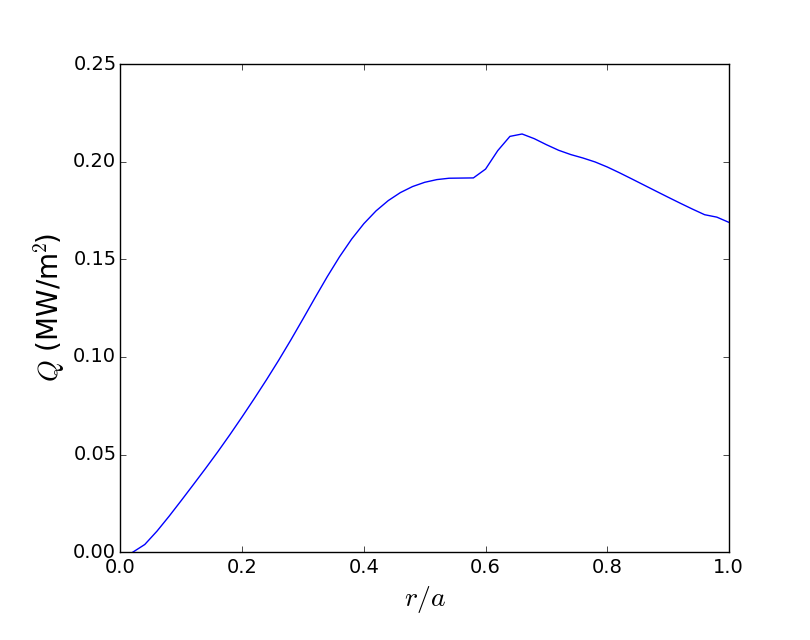
\includegraphics[width=0.7\textwidth]{turbHeatFlux.png}
\caption{\label{fig:turbHeatFlux} Heat flux $Q$ calculated with input heating and fusion rate profiles from TRANSP and TSC.}
\end{figure}

We estimate $\tau^{\text{turb}} = - \nabla \cdot \Pi_{\text{int}} \sim -\Pi_{\text{int}}/a$ using 
\begin{gather}
\Pi_{\text{int}} \sim \frac{\rho_{\theta} \widetilde{\Pi}(\nu_*) Q \langle R \rangle}{v_{ti} L_T}.
\end{gather}
The quantity $\tau^{\text{turb}}$ is shown in figure \ref{fig:alltorque}.

\FloatBarrier

\section*{Acknowledgements}
The authors would like to thank F. Parra, J. Hillesheim, J. Lee, and H. Smith for helpful input and discussions. This work was supported by the US Department of Energy through grants DE-FG02-93ER-54197 and DE-FC02-08ER-54964. The computations presented in this paper have used resources at the National Energy Research Scientific Computing Center (NERSC). 

\bibliography{ITERNTV}

\end{document}
